\section{Hipster: Implementation and Use}
\label{sec:hipster}

In this section we give an overview of Hipster, and show how it can be used both in theory exploration mode and in proof mode, to find lemmas relevant for a particular proof attempt. An overview of Hipster is shown in figure \ref{fig:hipster}. 

\begin{figure}[htbp]
\begin{center}
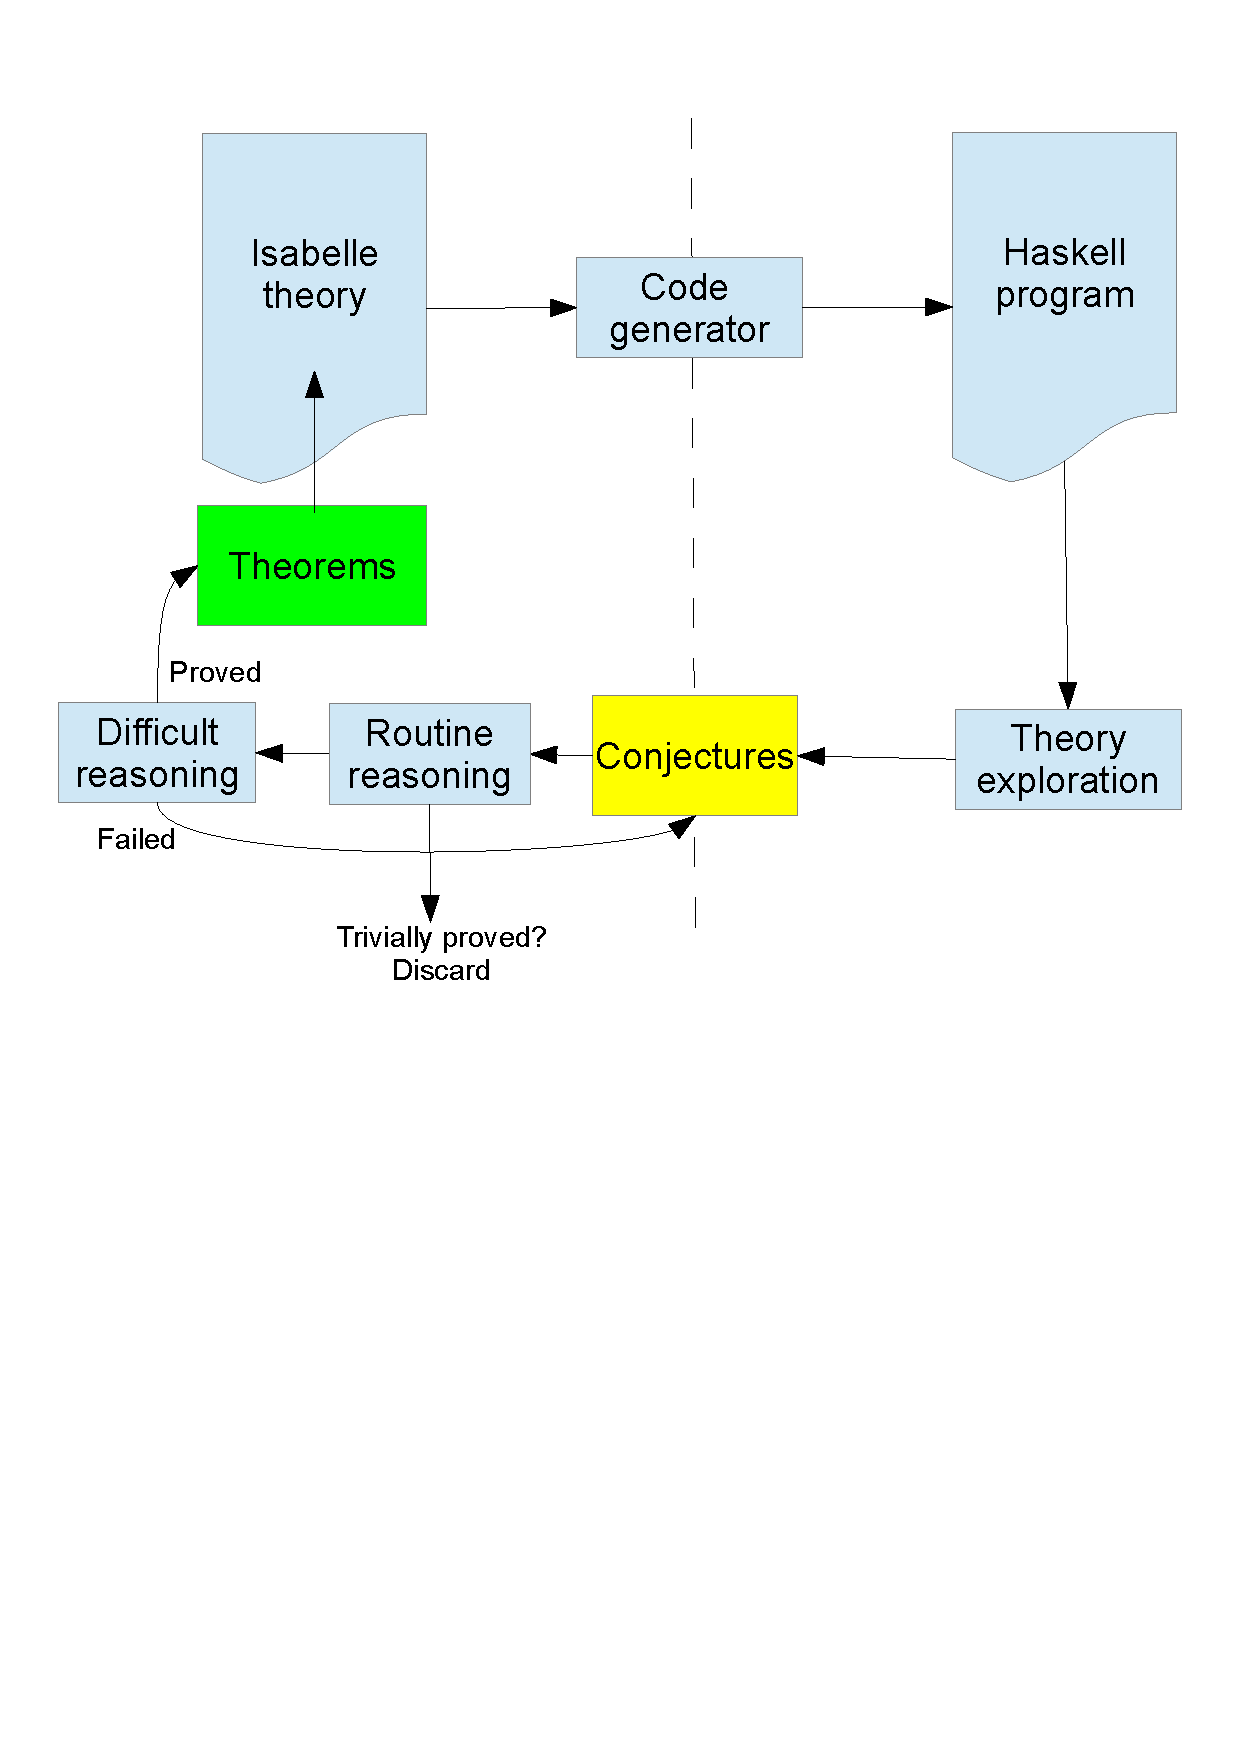
\includegraphics[scale=0.45]{hipster}

\caption{Overview of Hipster}
\label{fig:hipster}
\end{center}
\end{figure}

Starting from an Isabelle theory, Hipster calls Isabelle's code generator \cite{codegen} to translate the given functions into a Haskell program. In order to use the testing framework from QuickCheck, as described in the previous section, we must however also post-process the Haskell file, adding \emph{generators}, which are responsible for producing arbitrary values used for evaluation and testing. We use generators automatically deduced by the Feat package \cite{feat}. Another important issue that need to be addressed at this stage is the differences in semantics for partial functions in Isabelle and Haskell. In order to avoid HipSpec missing equations that hold in Isabelle, but not in Haskell, we had to modify the translation of partial functions. This is explained in more detail in section \ref{sec:partial}.

Once the Haskell program is in place, we run theory exploration and generate a set of equational conjectures, which HipSpec orders according to generality. More general equations are preferred, as we expect these to be more widely applicable as lemmas. In previous work on HipSpec, the system would at this stage apply induction on the conjectures and send them off to some external prover. Here, we instead import them back into Isabelle as we wish to produce checkable LCF-style proofs for our conjectures. 

The proof procedure in Hipster is parametrised by two tactics, one for easy or \emph{routine reasoning} and one for \emph{difficult reasoning}. In the examples below, we use Isabelle's simplifier followed by first-order reasoning by Metis as \emph{routine reasoning}, and a tactic performing structural induction followed by simplification and first-order reasoning as \emph{difficult reasoning}. Both tactics have access to the theorems proved so far, and hence gets stronger as the proof procedure proceed through the list of conjectures. As there are rather many conjectures produced by theory exploration, we do not want to present them all to the user, but rather select the most interesting ones, which are difficult to prove. Those that follow only by routine reasoning are filtered out. 
Depending on the theory and application we can change these tactics to suit our needs. If we want Hipster to produce fewer or more lemmas, we can choose a stronger or weaker tactic, allowing for flexibility.  

The order in which Hipster tries to prove things matter. As we mentioned, it will try more general conjectures first, with the hope that they will be useful to filter out many more specific routine results. Occasionally though, a proof will fail as a not yet proved lemma is required. In this case, the failed conjecture is added back into the list of open conjectures and retried later, provided that at least one new lemma has been proved in the meantime to ensure progress and termination. Hipster terminates when it either runs out of open conjectures, or when it does not make any more progress. 

\subsection{Theory Exploration Mode}
In this example we look at a theory about binary trees, with data stored at the leaves:
\begin{verbatim}
datatype 'a Tree = 
  Leaf 'a 
  | Node 'a Tree  'a Tree
\end{verbatim}

 
\subsection{Proof Mode}
The following example is about a compiler to a stack machine for a toy language with generic types of expressions\footnote{This example a slight variation of that in \S3.3 in the Isabelle tutorial \cite{isabelle}. It had to be modified as our generators on the Haskell side does not support generation of values for datatype constructors involving higher-order arguments)}. Expressions in the language are built from constants (\texttt{Cex}), values (\texttt{Vex}) and binary operators (\texttt{Bex}): 
\begin{verbatim}
datatype ('c, 'v, 'b) expr =
  Cex 'c |
  Vex 'v |
  Bex "'b" "('c,'v,'b) expr" "('c,'v,'b) expr"
\end{verbatim}
The types of variables, values and binary operators are not fixed, but given by type parameters \texttt{'c}, \texttt{'v} and \texttt{'b}. 
To evaluate an expression, we define a function \texttt{value}, parametrised by a lookup function for binary operators and an environment mapping variables to values:
\begin{verbatim}
fun value::('b =>'c =>'c =>'c) => ('v =>'c) => ('c,'v,'b) expr =>'c
where
  "value getBinop env (Cex c) = c" |
  "value getBinop env (Vex v) = env v" |
  "value getBinop env (Bex b e1 e2) = 
    (getBinop b) (value getBinop env e1) (value getBinop env e2)"
\end{verbatim}
A program for our stack machine consists of four instructions:
\begin{verbatim}
datatype ('c, 'v, 'b) program =
  Done
  | Const 'c "('c, 'v, 'b) program"
  | Load 'v  "('c, 'v, 'b) program"
  | Apply 'b "('c, 'v, 'b) program"
\end{verbatim}
A program is either empty (\texttt{Done}), or consists of one of the instructions \texttt{Const}, \texttt{Load} or \texttt{Apply}, followed by the remaining program. 